\chapter{Previous work} \label{sec:previous_work}
\section{Food localization}

%% Color and edge segmentation
%% 11.1

A way to localize food is based on edge detection and color segmentation.

In \cite{Thendral2014a}, the authors describes and compare these two methods to localise an orange in a picture. It applied these methods on a small dataset of 20 orange images (only one orange per image), with different lighting conditions and backgrounds (pictures are taken from the Internet).
In more details, the edge-based segmentation apply the canny-edge segmentation, then apply non-maximum suppression to eliminate noises. Then, each pixels are classified.
The colour-based segmentation normalised the lightning condition with a gaussian low-pass filter, convert the RGB image into a $L * a * b$
\begin{enumerate}
    \item gaussian low pass filter to normalize the lightning condition
    \item convert the image from RGB representation to $L * a * b$
    \item use the $a$ channel to classify each pixel as \enquote{fruit} or \enquote{non-fruit}
    \item remove small object
    \item fill the binary image regions and holes
\end{enumerate}
For orange detection, the color segmentation has an higher accuracy. Yet, it is very hard to generalise this method.

%% Circle
%% 2.2 (partial) + 6.3 + \cite{Dehais2015} ?

An other method for food detection relies on circle detection. Indeed, food items are often served in a round shape container such as a bowl, a pan or a plate.

In \cite{Matsuda2012a}, the authors propose a food recognition system to identify food items of a picture. The first step is to detect potential region with multiple object detection algorithms. Then, for these regions, several feeatures are extracted and used to feed SVM with multiple kernel learning method. To detect candidate regions, the authors use:
\begin{itemize}
    \item Felzenszwalb’s deformable part model (DPM): based on Histogram of Oriented Gradients (HOG). Multiple HOGs are
    \item circle detector: convert the image to a gray-scale image, extracts contour by the Canny Edge Detector and detect circle by the Hough Transform
    \item JSEG region segmentation: segmente region based on color. Only keep circular regions.
    \item whole image: for image with one large dish
\end{itemize}
Then, it agregates all the candidate region to get bounding box of each food item.
For evaluation, the authors build a new dataset composed of 100 categories with their associated bouding boxes for a total of 9060 images. For multiple food item images, they obtain 55.8 \% classification rate and 68.9 \% for single food item pictures.

In \cite{Wazumi2011}, the authors desribe their use of the Hough transformation to detect circle (they constitutes the food region).

%% CNN
%% DCNN: * ? + 9.1 (in food intake)

\section{Food recognition}

Food recognition

Using SVM:

Local using BOW: 3.3
gloabal feature:
Color and texture description: 
Spatial pyramid:

Mix of several features:

In \cite{Zhu2015}, the authors develop a mobile application to keep food records of a user that is taking pictures of one's meal. Their method can detect multiple food items in one picture. They use a color marker as an illumination and size indicator.

When the user upload a picture, it is segmented, then classified by a backend server. The estimation are sent back to the user for confirmation.

Their method is named "multiple hypotheses segmentation and classification (MHSC)". It is an iterative method composed of a segmentation, description (extraction of features) and classification step.

For segmentation, the authors first detect salient region, using Canny edge and color distribution to reject background. Then, they apply a multiscale segmentation using normalized cut. Small segmented regions are discarded.

On the selected region, the authors used a mixed of global descriptors (first and second moment of each channel for RGB, YCbCr, L*a*b*, and HSV color spaces, first and second moment of the entropy in RGB, predominant color describtor, entropy and two first moments of the Gradient Orientation Spatial-Dependence Matrix, entropy categorization and fractal dimension estimation and estimation of the fractal dimension of the response of different gabor filter) with local feature (multi Bag-Of-Words using SIFT for RGB, SURF for RGB, SIFT for each channel of the RGB representation and steerable filters).

Each of the 12 descriptor, global and local, is classified independantly and assigned a confidence score. A late fusion function (either maximum confidence score or majority vote) is used  to decide the final class. For clasification, the authors use K-NN and SVM.

If the total score is inferior to a certain threshold, the overral process is repeated. The confidence score of the previous step is used to improve the segmentation.

Applied on a dataset composed of 83 labels (79 food classes plus \enquote{utensils}, \enquote{glasses}, \enquote{plates}, and \enquote{plastic cups} classes), each class having at least 30 images, they obtain a top-8 accuracy of 75 \%, using K-NN with the maximum confidence score.

%% DCNN
%% 2.3

In \cite{Kawano2014}, the authors use a pre-trained DCNN as a feature descriptor. The DCNN, nammed OverFeat, can be found  \href{http://cilvr.nyu.edu/doku.php?id=code:start}{here} and was trained on ImageNet.
The authors add more conventional image features to have: 
\begin{enumerate}
    \item HOG (more exactly, RootHog that is “an element-wise square root of the L1 normalized HO”) (8 orientations per block of 2 * 2)
    \item color patches (mean and variance values of  RGB value of pixels from each of 2*2  block)
    \item Deep convolutional neural network last two layers
\end{enumerate}
The three descriptors are then encoded in a fisher vector.
Using SVM, they obtain 72\% of accuracy for UEC-FOOD 100.

\begin{enumerate}
    \item Feature:
    
    
    \item Encoding: Fisher vector
\end{enumerate}

\section{Food intake estimation}

%% Food Log

FoodLog \footnote{\url{http://www.foodlog.jp}} is a website that enables the user to upload pictures of its daily meals to be archived and processed. The goal of this application is to assist the user to keep notes of their meals and balance the nutritional values coming from different kinds of food.

In \cite{Kitamura2008}, the images containing food items are identified by exploiting features related to the HSV and RGB colour domains, as well as the shape of the plate. A SVM classifier is trained to detect food images. More specifically, the images are divided in 300 blocks and each block is classified as \enquote{non-food} (discarded block) or one of the nutritional categories described in the \enquote{MyPyramid} model \footnote{\url{http://www.mypyramid.gov}}.

MyPyramid \cite{MyPyramid} was designed by the United State Departement of Agriculture \textit{USDA} in 2005 and was replaced in 2011 by \enquote{MyPlate} \footnote{\url{http://www.choosemyplate.gov}} \cite{MyPlate}. This dietary model is composed of 5 kinds of food: grains, vegetable, meals and beans, milk and fruit. For each group, a recommended intake per day is associated, Fig. \ref{fig:my_pyramid}. Quantity is categorized by \enquote{servings} \textit{SV}, making it simpler to compute and keep log.

\begin{figure}
    \centering
    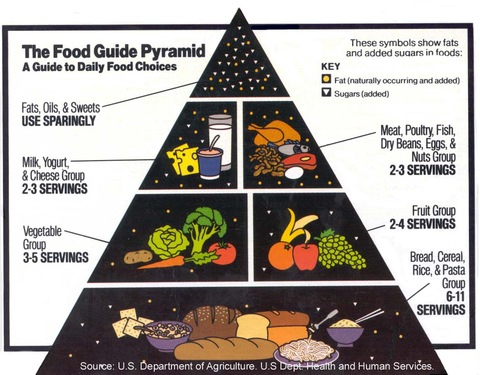
\includegraphics[scale=0.8]{img/my_pyramid.jpg}
    \caption{USDA MyPyramid original logo}
    \label{fig:my_pyramid}
\end{figure}

In \cite{Aizawa2013} the Support Vector Machine is replaced by a Bayesian Framework \textit{BF}.
The BF is based on the Gaussian Naive Bayesian (suppose independence between every pair of features and the distribution of each feature is assumed to be Gaussian). The BF takes into account the estimation using color moments and Bag-Of-Feature of SIFT, the prior distribution and the mealtime category (breakfast, lunch and dinner).

In \cite{Kagaya2014}, the authors use a Convolutional Neural Network \textins{CNN} to detect and classify food from a small subset of image loaded in the FoodLog system. Compared to the other conventional methods (use of a feature descriptor such as Bag-of-Words with a classifier, e.g. SVM) described previously, the CNN showed a significantly higher accuracy.

%% Others

An other method to estimate the food intake is to evaluate the food volume.

In \cite{Chen2012}, the authors presents a method that use the depth information of the picture. Once the food has been classified, the area of the food container (bowl, plate) and the depth value of the contained food is computed to obtain the food volume.
Yet, this technique is still limited as it can only be used for non-transparent food, i.e it can't detect some food item such as water or cooked rice, and force the user to have a depth camera (such as Kinect).

In \cite{Almaghrabi2012a}, the authors presents a novel food recognition system that is able to estimate of the nutrition intake. Moreover, they develop a mobile application to easily take pictures and keep track of the user's diet.
To measure the food intake, authors compare before and after eating pictures and use the thumb as the calibration system (it supposes a one-time calibration to know the size of the thumb of the user).
The process to show the intake is:
\begin{enumerate}
    \item the user takes food pictures
    \item get the contour of each picture
    \item recognition of the food using color, shape and size features with SVM.
    \item volume calculation, that is computed in two steps:
    \begin{enumerate}
        \item user takes a picture from above. Then, the food shape is divided into known shape (rectangle, circle, triangle ...) to compute the area.
        \item user takes a second picture from the side. This is used to compute the height of the food and calculate the overall volume.
    \end{enumerate}
    The system assumes that the plate is white and round.
    \item use a nutrition database to obtain the average calories
\end{enumerate}
If the user hasn't eaten everything, the entire must be repeated.
The drawbacks of this method is the user have to take several pictures, with one's thumb each time and it has been tested with a limited set of simple food types.

%% Food Cam ?